\newpage
\section{Cơ chế xác thực và phân quyền}

\subsection{Luồng xác thực}

Xác thực là quá trình kiểm tra và xác minh danh tính của người dùng trước khi cho phép truy cập vào hệ thống. Trục tích hợp dữ liệu sử dụng JSON Web Token (JWT) kết hợp với thư viện Passport.js để thực hiện cơ chế xác thực phi trạng thái (\textit{stateless}).

Quy trình xác thực diễn ra theo các bước sau:

\begin{enumerate}
    \item Người dùng gửi yêu cầu đăng nhập kèm theo tên đăng nhập và mật khẩu đến điểm cuối API \texttt{POST /auth/login}.

    \item Dịch vụ xác thực truy vấn bảng \texttt{users} trong PostgreSQL để tìm người dùng theo tên đăng nhập. Mật khẩu được xác minh thông qua hàm \texttt{bcrypt.compare} bằng cách đối chiếu với giá trị băm đã lưu trong cột \texttt{passwordHash}.

    \item Nếu thông tin hợp lệ, hệ thống khởi tạo một mã truy cập JWT với phần dữ liệu tải trọng (payload) chứa các thông tin sau:

    \begin{itemize}
        \item \texttt{sub}: Định danh người dùng (ID).
        \item \texttt{username}: Tên đăng nhập.
        \item \texttt{role}: Vai trò của người dùng (\texttt{admin} | \texttt{reader} | \texttt{writer}).
        \item \texttt{roleSettings}: Cấu hình phạm vi quyền hạn dưới định dạng JSON (được trình bày chi tiết tại Mục~\ref{subsec:authorization}).
    \end{itemize}

    \item Mã truy cập được ký số bằng khóa bí mật \texttt{JWT\_SECRET} và có thời gian tồn tại được quy định thông qua biến môi trường \texttt{JWT\_EXPIRES\_IN}.

    \item Sau khi nhận được mã truy cập, người dùng đính kèm mã này vào mọi yêu cầu truy xuất tài nguyên tiếp theo. Hệ thống hỗ trợ hai hình thức truyền mã truy cập:

    \begin{itemize}
        \item Qua Tiêu đề HTTP (HTTP Header):
\begin{verbatim}
Authorization: Bearer <token>
\end{verbatim}
        \item Qua tham số truy vấn (URL Query - áp dụng cho các kết nối luồng dữ liệu liên tục như SSE):
\begin{verbatim}
GET /integration/stream-logs?token=<token>
\end{verbatim}
    \end{itemize}
\end{enumerate}

Việc sử dụng JWT giúp hệ thống tuân thủ hoàn toàn kiến trúc phi trạng thái — máy chủ không cần lưu trữ thông tin phiên làm việc (session); mọi thông tin cần thiết để xác thực và phân quyền đều được nhúng gọn bên trong mã thông báo.

\begin{figure}[!htp]
    \centering
    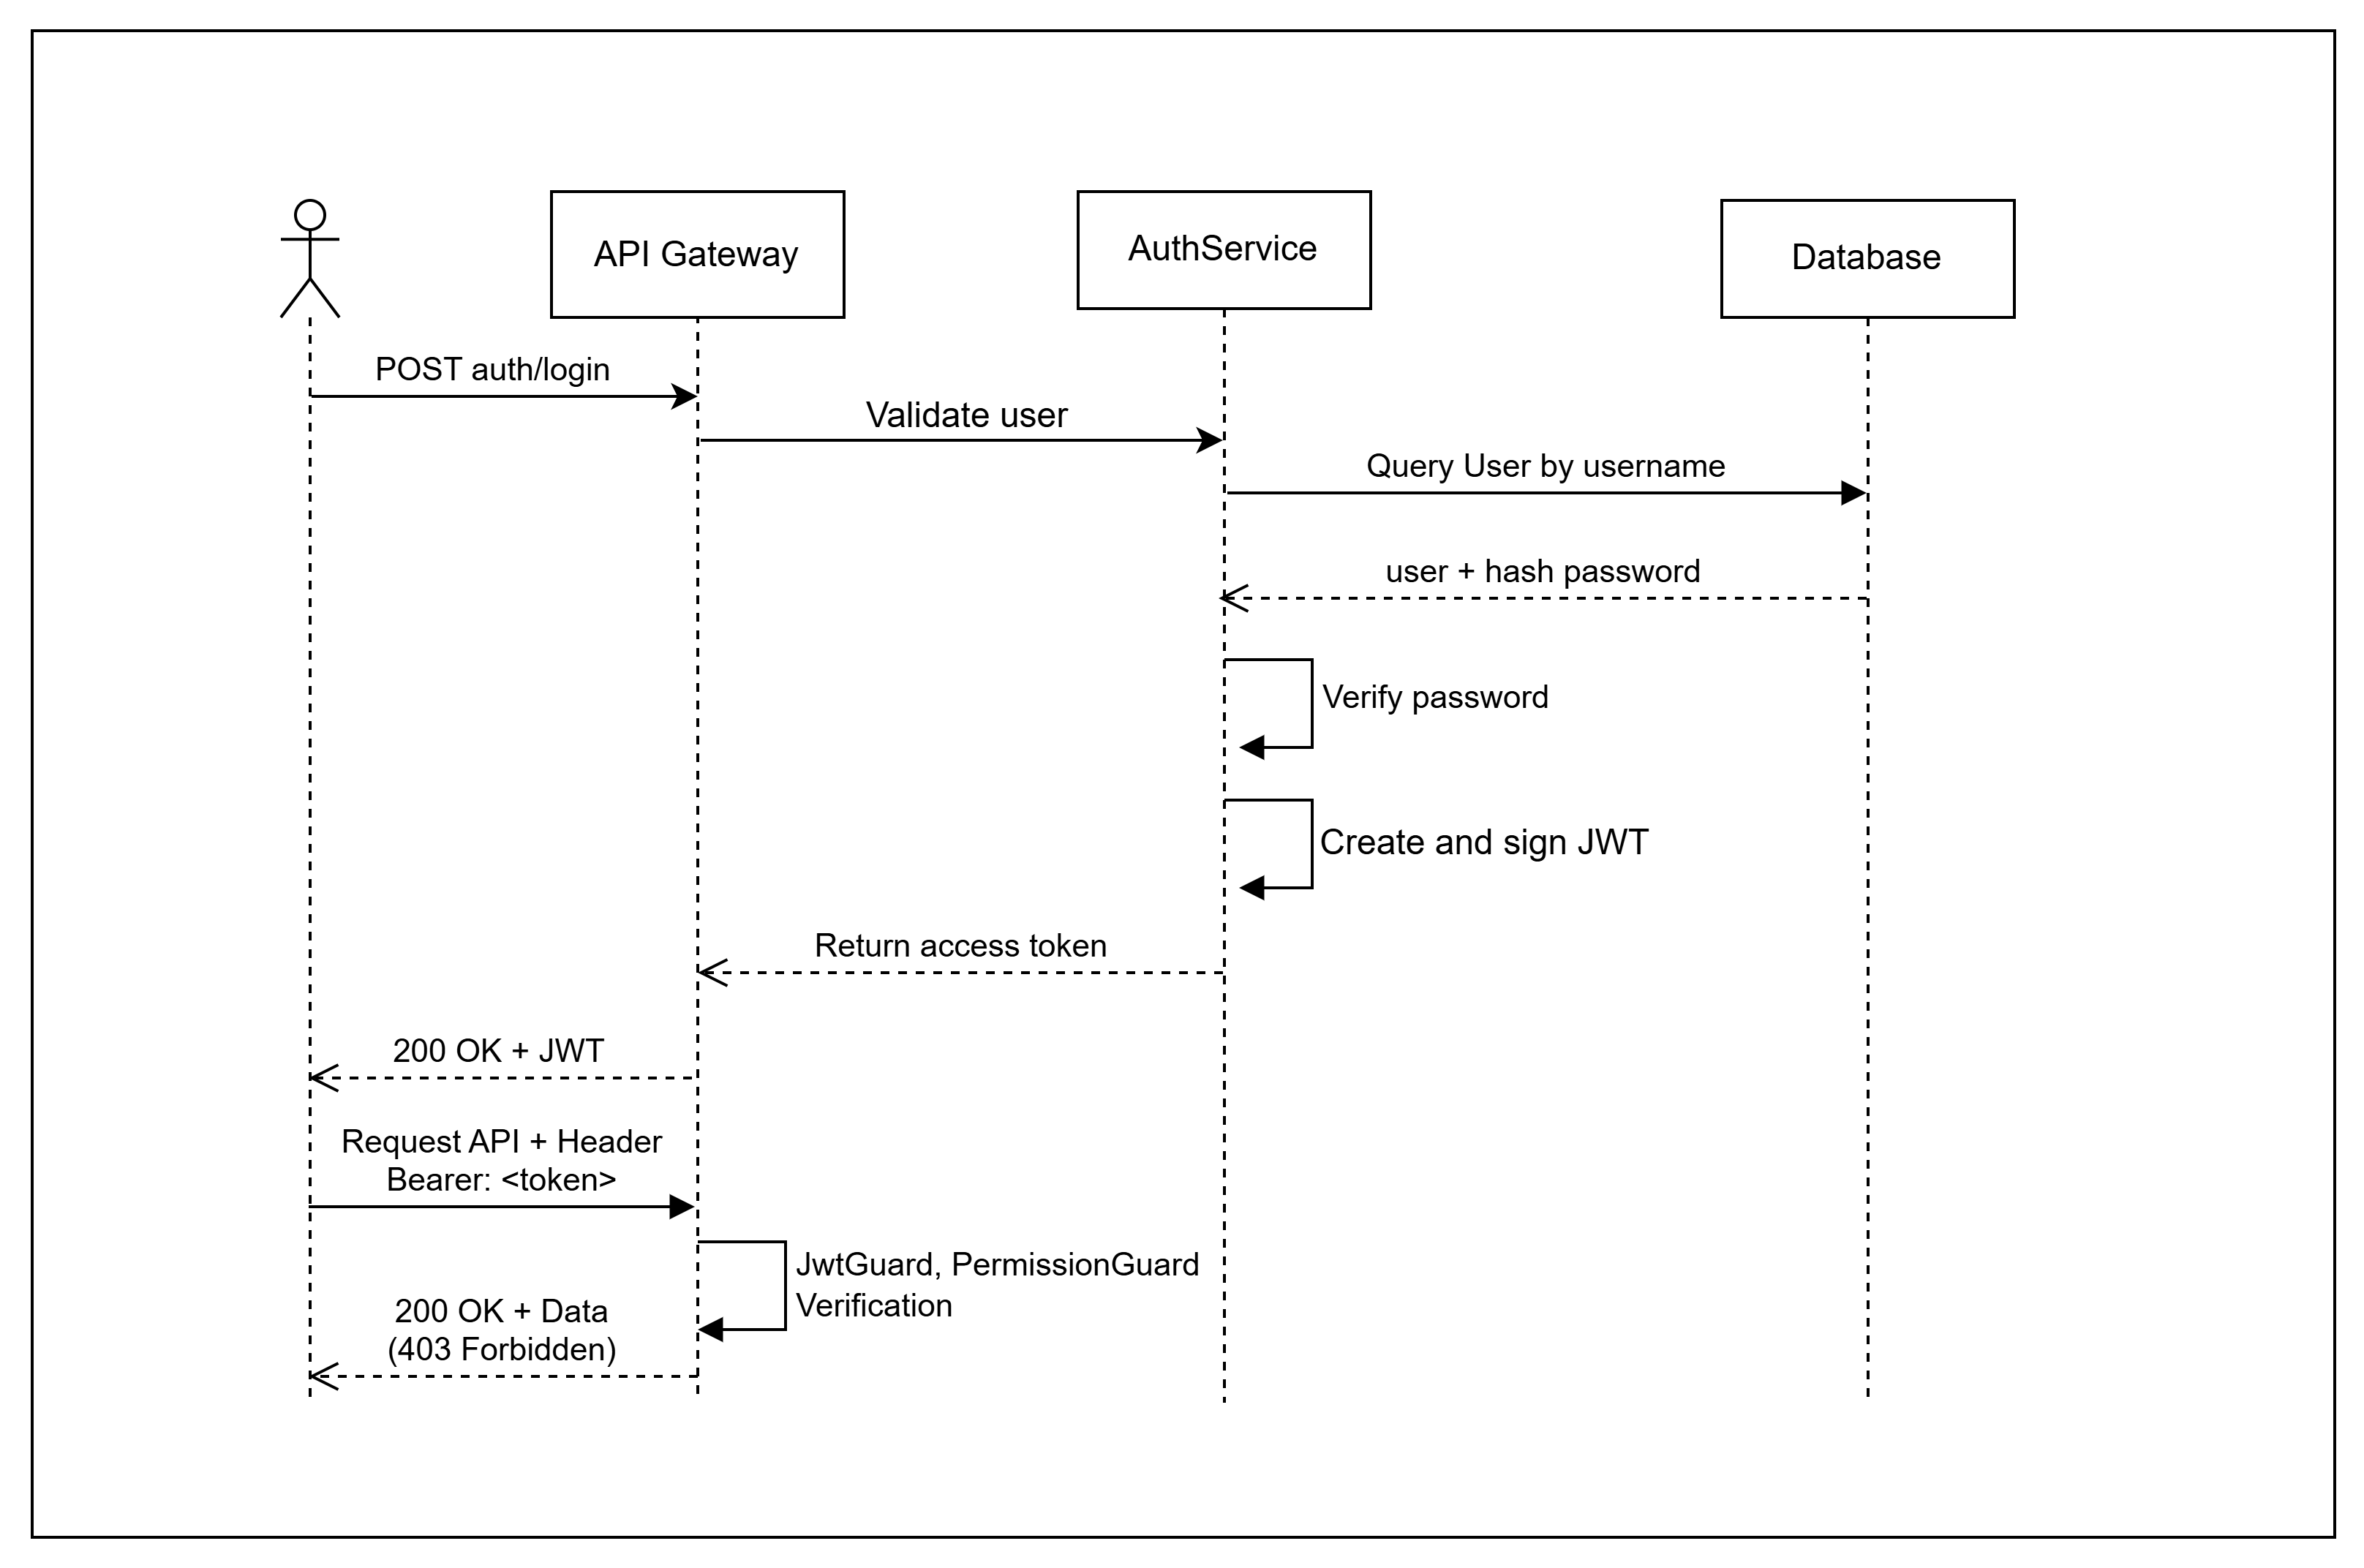
\includegraphics[width=1\linewidth]{graphics/authentication.png}
    \caption{Luông xác thực và kiểm tra quyền truy cập}
    \label{fig:authentication_flow}
\end{figure}

\subsection{Luồng phân quyền}
\label{subsec:authorization}

Sau khi hệ thống xác thực người dùng thành công, luồng yêu cầu tiếp tục đi qua hai lớp bảo vệ độc lập để thực hiện kiểm tra quyền truy cập một cách tuần tự.

\subsubsection{Lớp 1 — Kiểm tra vai trò (\texttt{RolesGuard})}

Hệ thống định nghĩa ba vai trò cố định, được lưu trực tiếp trên bảng \texttt{users}:

\begin{itemize}
    \item \textbf{\texttt{admin}}: Quản trị viên hệ thống, có toàn quyền truy cập tài nguyên và được đặc cách bỏ qua mọi bước kiểm tra phân quyền phía sau.
    \item \textbf{\texttt{reader}}: Người dùng chỉ có quyền đọc dữ liệu trong phạm vi được chỉ định.
    \item \textbf{\texttt{writer}}: Người dùng có quyền cả đọc và ghi dữ liệu trong phạm vi được chỉ định.
\end{itemize}

\texttt{RolesGuard} chịu trách nhiệm đọc danh sách vai trò cho phép từ bộ trang trí (\textit{decorator}) \texttt{@Roles()} gắn trên các trình điều khiển (controller) hoặc từng điểm cuối cụ thể. Sau đó, hệ thống đối chiếu với trường \texttt{role} lấy từ tải trọng JWT. Nếu không khớp, yêu cầu sẽ bị từ chối ngay lập tức với mã lỗi 403 Forbidden.

\subsubsection{Lớp 2 — Kiểm tra phạm vi bảng (\texttt{PermissionsGuard})}

Ngoài vai trò, mỗi người dùng (ngoại trừ \texttt{admin}) được cấp một cấu hình \texttt{roleSettings} lưu dưới định dạng JSON trong cơ sở dữ liệu:

\begin{lstlisting}[caption={Cấu trúc cấu hình roleSettings}]
{
  "writeScopes": ["^tcns_.*", "^dm_gioi_tinh$"],
  "readScopes":  ["^nguoi_hoc$", "^dm_.*"]
}
\end{lstlisting}

Mỗi phần tử trong mảng \texttt{writeScopes} và \texttt{readScopes} là một biểu thức chính quy (\textit{regular expression}) dùng để so khớp với tên bảng được truyền qua tham số động \texttt{:table} của URL yêu cầu. Logic kiểm tra được thực thi như sau:

\begin{itemize}
    \item \textbf{Admin}: Bỏ qua hoàn toàn bước kiểm tra này.
    \item \textbf{Thao tác đọc} (Phương thức \texttt{GET}):
        \begin{itemize}
            \item \texttt{reader}: Tên bảng phải khớp với ít nhất một biểu thức trong \texttt{readScopes}.
            \item \texttt{writer}: Tên bảng phải khớp với ít nhất một biểu thức trong \texttt{readScopes} \textbf{hoặc} \texttt{writeScopes}.
        \end{itemize}
    \item \textbf{Thao tác ghi} (Phương thức \texttt{POST}, \texttt{PUT}, \texttt{PATCH}, \texttt{DELETE}): Chỉ tài khoản \texttt{writer} được phép thực hiện, và tên bảng bắt buộc phải khớp với ít nhất một biểu thức trong \texttt{writeScopes}.
\end{itemize}

Việc ứng dụng biểu thức chính quy mang lại tính linh hoạt rất cao trong cấu hình. Ví dụ: biểu thức \texttt{\^{}tcns\_.*} cấp quyền truy cập hàng loạt cho toàn bộ các bảng có tiền tố \texttt{tcns\_}, trong khi biểu thức \texttt{\^{}dm\_gioi\_tinh\$} giới hạn quyền truy cập chặt chẽ vào đúng một bảng duy nhất.

\subsection{Cơ chế cấp lại mã truy cập}

Khi mã truy cập ngắn hạn hết hiệu lực, người dùng chỉ cần gửi lại mã cũ đến điểm cuối \texttt{POST /auth/refresh-token}. Hệ thống sẽ xác minh chữ ký và tính toàn vẹn của mã thông qua phương thức \texttt{jwtService.verify()}, sau đó trích xuất dữ liệu gốc để ký lại và phát hành một mã truy cập hoàn toàn mới.

Cơ chế này giữ được sự tối giản về mặt logic và không yêu cầu phải lưu trữ thêm \textit{Refresh Token} trong cơ sở dữ liệu, đáp ứng tốt yêu cầu về mô hình phi trạng thái của toàn bộ hệ thống.

\begin{figure}[!htp]
    \centering
    
\includegraphics[width=1\linewidth]{graphics/refresh_token.png}
    \caption{Luồng xử lý cấp lại mã truy cập (Refresh Token)}
    \label{fig:refresh_token_flow}
\end{figure}

\subsection{Cấu trúc cơ sở dữ liệu phục vụ xác thực và phân quyền}

Khác với mô hình kiểm soát truy cập dựa trên vai trò truyền thống (RBAC - Role-Based Access Control) thường đòi hỏi nhiều bảng trung gian phức tạp, hệ thống trục tích hợp đã hợp nhất toàn bộ thông tin xác thực và phân quyền vào một bảng duy nhất:

\begin{itemize}
    \item \textbf{\texttt{users}}: Lưu trữ thông tin định danh bao gồm tên đăng nhập, mật khẩu đã băm (\texttt{passwordHash}), họ tên, thư điện tử, kết hợp với vai trò hệ thống (\texttt{role}) và cấu hình phạm vi quyền (\texttt{roleSettings}).
\end{itemize}

Lối thiết kế này đạt được sự cân bằng tối ưu giữa tính đơn giản và độ linh hoạt: trường vai trò kiểu liệt kê (enum) đảm bảo tính nhất quán cho các thao tác cấp cao, trong khi trường \texttt{roleSettings} lưu dạng JSON cho phép tùy biến phạm vi quyền chi tiết đến từng bảng cụ thể mà không cần phải thực hiện di cư dữ liệu (migration) làm thay đổi cấu trúc bảng.